% ============================================================================
% HACE: Addressing Viability Failure in Sequential RL
%       with Homeostatic Auxiliary Rewards
%
% STATUS: PI Review Draft — NOT for submission.
% PURPOSE: Show existing work, get feedback, identify gaps.
%
% To compile:
%   cd hace_draft/
%   pdflatex main.tex && pdflatex main.tex
% ============================================================================

\documentclass{article}
\usepackage[preprint]{neurips_2023}

% ── Packages ─────────────────────────────────────────────────
\usepackage{amsmath,amssymb,amsfonts}
\usepackage{booktabs}
\usepackage{graphicx}
\usepackage{hyperref}
\usepackage{xcolor}
\usepackage{enumitem}
\usepackage{multirow}
\usepackage{caption}
\usepackage{subcaption}

% ── Draft commands ───────────────────────────────────────────
\newcommand{\todo}[1]{\textcolor{red}{\textbf{[TODO: #1]}}}
\newcommand{\note}[1]{\textcolor{blue}{\textbf{[NOTE: #1]}}}
\newcommand{\picomment}[1]{\textcolor{purple}{\textbf{[PI Q: #1]}}}

% ── Notation shortcuts ───────────────────────────────────────
\newcommand{\setpoint}{H^*}
\newcommand{\energy}{E}
\newcommand{\drive}{d}
\newcommand{\rwd}{r}
\newcommand{\hace}{\textsc{Hace}}

% ============================================================================
\title{HACE: Addressing Viability Failure in Sequential RL\\
with Homeostatic Auxiliary Rewards}

\author{
  Ziyu Kong \quad Shihang Gui \quad Ruth Ukubay \quad Meiyi Song \\
  Department of Computer Science \\
  Brown University, Providence, RI, USA \\
  \texttt{\{ziyu\_kong, shihang\_gui, ruth\_ukubay, meiyi\_song1\}@brown.edu}
}

\begin{document}
\maketitle

% ============================================================================
\begin{abstract}
% ============================================================================

Continual reinforcement learning (CRL) research has focused primarily on
\emph{catastrophic forgetting}---the tendency for neural networks to lose
previously acquired skills when adapting to new tasks. In embodied settings
where agents must manage shared physiological resources such as energy,
however, we identify a complementary and equally critical failure mode:
\emph{viability failure}, wherein agents deplete internal resources and die
before they can learn a new task. We argue that established CRL techniques
such as Elastic Weight Consolidation (EWC) and Experience Replay (ER),
which operate at the weight or data level, are structurally incapable of
addressing viability failure because it is a \emph{reward and survival}
problem, not a parameter-preservation problem. We propose \hace{}
(Homeostatic Auxiliary for Continual Environments), a simple, task-invariant
auxiliary reward based on homeostatic drive reduction that incentivizes
energy management without requiring task-specific engineering.
We evaluate \hace{} alongside 8 baseline agents---including EWC, ER, and L2
regularization---on a 10-task sequential gridworld benchmark with 3 task
orderings and 2 boundary modes. Preliminary results demonstrate that
\hace{} agents maintain viability across task transitions, achieve
significantly higher boundary solvability, and exhibit stronger forward
transfer, while traditional CRL methods alone fail to prevent agent death
at task boundaries. Our findings suggest that viability maintenance
is an essential and overlooked prerequisite for continual embodied learning.

\end{abstract}

% ============================================================================
\section{Introduction}
\label{sec:intro}
% ============================================================================

Reinforcement learning agents deployed in sequential or continual settings
must adapt to changing objectives without losing previously learned capabilities.
The dominant research paradigm in continual RL (CRL) frames this challenge
almost exclusively as \emph{catastrophic forgetting}---the well-documented
tendency for neural network parameters to overwrite old knowledge when trained
on new tasks~\citep{Parisi2019,kirkpatrick2017,continualworld2021}. A rich
toolkit of methods has emerged to combat forgetting: weight regularization
(EWC~\citep{kirkpatrick2017}), experience replay~\citep{rolnick2019}, progressive
architectures~\citep{rusu2016}, and policy distillation. These methods are
evaluated almost exclusively on whether old-task performance degrades after
new-task training.

We argue that this singular focus on forgetting obscures an equally critical
failure mode that emerges naturally in \emph{embodied} sequential settings:
\textbf{viability failure}. When an agent operates in an environment with
shared physiological constraints---such as an internal energy variable that
depletes with each action---the transition between tasks can be lethal. An agent
that completes Task~$T_i$ with minimal remaining energy may arrive at
Task~$T_{i+1}$ without sufficient resources to survive long enough to learn.
No amount of EWC regularization or replayed transitions can save an agent
that dies in the first three steps of a new task.

Consider a concrete example from our benchmark. An agent trained on
\textsc{Conservation} (high step cost, must be efficient) transitions to
\textsc{Sprint} (very short time limit, must be fast). Under carryover
boundary conditions---where energy is not reset between tasks---a task-only
agent that learned conservative movement arrives at \textsc{Sprint} with
critically low energy and zero time to explore. It dies immediately. EWC
preserves the \textsc{Conservation} weights perfectly, but those weights
are useless if the agent cannot survive.

This paper makes three contributions:

\begin{enumerate}[leftmargin=*,topsep=2pt,itemsep=1pt]
  \item We formally identify \textbf{viability failure} as a distinct failure
        mode in continual embodied RL, separate from catastrophic forgetting,
        and show that traditional CRL methods are structurally unable to
        address it (Section~\ref{sec:viability}).

  \item We propose \textbf{\hace{}} (Homeostatic Auxiliary for Continual
        Environments), a simple, task-invariant auxiliary reward based on
        biological homeostatic drive reduction that incentivizes energy
        management across all tasks without task-specific
        engineering (Section~\ref{sec:hace}).

  \item We design a \textbf{10-task sequential gridworld benchmark} with
        12 structurally diverse tasks, 3 curated task orderings, 9 agent
        variants (including EWC, ER, and oracle baselines), and 2
        boundary modes (reset/carryover) that enables systematic study of
        both forgetting and viability (Section~\ref{sec:benchmark}).
\end{enumerate}

Our preliminary results (Sections~\ref{sec:pilot}--\ref{sec:factorial})
demonstrate that \hace{} agents maintain viability across task boundaries,
achieve higher boundary solvability, and exhibit stronger forward transfer
than both task-only agents and standard CRL baselines. Critically, \hace{}
is \emph{orthogonal} to forgetting-prevention methods: combining \hace{}
with EWC (Agent~I in our catalog) addresses both failure modes
simultaneously.

% ============================================================================
\section{Related Work}
\label{sec:related}
% ============================================================================

\subsection{Continual Reinforcement Learning}

The CRL literature focuses on preventing catastrophic forgetting when an
agent's task changes over time. Elastic Weight Consolidation
(EWC;~\citep{kirkpatrick2017}) slows updates to parameters deemed important
for previous tasks via a Fisher-weighted penalty. Experience Replay
(ER;~\citep{rolnick2019}) retains a buffer of past transitions and
interleaves them during training on new tasks. Progressive Neural
Networks~\citep{rusu2016} freeze old columns and add new capacity per task,
while policy distillation approaches~\citep{rusu2015} transfer knowledge
via soft targets.

These methods have been benchmarked extensively on Continual
World~\citep{continualworld2021} and CORA~\citep{cora2022}, predominantly
in robotic manipulation settings where episode termination is not
affected by resource constraints. Our work highlights that this evaluation
paradigm systematically misses viability failure because these benchmarks
lack shared physiological dynamics.

\subsection{Homeostatic Reinforcement Learning}

Homeostatic RL (HRRL) formalizes reward as deviation reduction from an
internal setpoint, grounding value in the agent's physiological
state~\citep{keramati2014}. Keramati and Gutkin show that HRRL produces
risk-averse and anticipatory behaviors in a single-task setting. Yoshida
extends this to deep RL~\citep{yoshida2018} and later connects HRRL to
meta-RL via recurrent adaptation~\citep{Yoshida}. Konidaris and Barto
propose adaptive motivational systems where internal drives guide
behavior~\citep{konidaris2006}.

However, all prior HRRL work studies single or slowly shifting
environments. No existing work tests whether homeostatic objectives
improve \emph{sequential task learning}, nor frames homeostasis as
an anti-viability-failure mechanism in CRL.

\subsection{Transfer and Multi-Task RL}

Successor features (SF;~\citep{Barreto}) enable transfer by decomposing
value into reusable dynamics representations and task-specific reward
weights. Generalized policy improvement selects the best available
behavior without retraining. Tomov et al.~\citep{Tomov} show that humans
reuse old policies in multi-task settings, and note that task descriptions
could be grounded in internal physiological states---an insight our work
directly operationalizes. Unlike SF-based methods, \hace{} requires no
task-specific feature engineering; the auxiliary reward is fixed and
universal.

\subsection{Auxiliary Rewards and Intrinsic Motivation}

Auxiliary rewards have been used to improve sample efficiency in RL:
pixel control~\citep{jaderberg2017}, reward prediction, and curiosity-driven
exploration~\citep{pathak2017}. \hace{} differs from these in that the
auxiliary signal is not designed for exploration or representation learning,
but for \emph{viability maintenance}---keeping the agent alive so that
primary task learning can proceed.

% ============================================================================
\section{Problem Formulation}
\label{sec:problem}
% ============================================================================

\subsection{Sequential Task Setting}

We consider an agent that must learn a sequence of tasks
$T_1, T_2, \ldots, T_n$, where all tasks share:
\begin{itemize}[leftmargin=*,topsep=1pt,itemsep=1pt]
  \item a common action space $\mathcal{A} = \{\text{up, down, left, right}\}$,
  \item an internal energy variable $\energy_t \in [0, \energy_{\max}]$ with
        per-step cost $c_{\text{step}}$,
  \item a terminal condition: $\energy_t \leq 0 \implies \text{death}$.
\end{itemize}

Tasks differ in grid size, hazard configurations, food placement, wall
layouts, gate mechanisms, step costs, and energy capacities (see
Table~\ref{tab:tasks}). Each task is trained for a fixed budget of
$K$ episodes. At task boundaries, the agent's network parameters are
retained (sequential learning), while energy is handled according to
the \emph{boundary mode}:

\begin{itemize}[leftmargin=*,topsep=1pt,itemsep=1pt]
  \item \textbf{Reset}: energy is reinitialized to the task's default
        $\energy_0$ at each boundary.
  \item \textbf{Carryover}: energy from the last episode of $T_i$
        carries over to the first episode of $T_{i+1}$, clamped to
        $[\energy_{\min}, \energy_{\max}^{(i+1)}]$.
\end{itemize}

The carryover mode is the ecologically realistic setting: a biological
agent cannot reset its metabolism. It is also the setting where viability
failure is most acute.

\subsection{Viability Failure}
\label{sec:viability}

\begin{definition}[Viability Failure]
An agent experiences \emph{viability failure} at task boundary $T_i \to T_{i+1}$
if, under the learned policy $\pi_i$, the expected energy at the end of
Task~$T_i$ is insufficient to sustain exploration in $T_{i+1}$:
\begin{equation}
  \mathbb{E}_{\pi_i}\!\left[\energy_{T_i}^{\mathrm{terminal}}\right]
  \;<\; \energy_{\mathrm{viable}}^{(i+1)}
\end{equation}
where $\energy_{\mathrm{viable}}^{(i+1)}$ is the minimum energy required to
reach any rewarding state in $T_{i+1}$.
\end{definition}

Under viability failure, the agent dies in the first few steps of the new
task with high probability. No gradient information about the new task is
obtained---the agent observes only a short sequence of death trajectories.
This differs fundamentally from catastrophic forgetting:

\begin{itemize}[leftmargin=*,topsep=1pt,itemsep=1pt]
  \item \textbf{Forgetting} is a \emph{parameter-level} problem: old
        weights are overwritten. Solutions operate on weights (EWC) or
        data (ER).
  \item \textbf{Viability failure} is a \emph{reward-level} problem: the
        agent never survives long enough to receive learning signal.
        Weight-level solutions are irrelevant---there is nothing to forget
        if nothing was learned.
\end{itemize}

\subsection{Why Traditional CRL Methods Cannot Fix Viability Failure}

EWC adds a penalty $\lambda \sum_i F_i (\theta_i - \theta_i^*)^2$ that
constrains parameter drift from the old task. This preserves old behavior
but does nothing to ensure the agent conserves energy. An EWC agent with
perfectly preserved \textsc{Reach} parameters will still die in
\textsc{Recharge} if it never learned to collect food.

Experience Replay interleaves old transitions during new-task training.
If the old transitions come from a task with different energy economics
(e.g., high initial energy), replaying them provides misleading energy
context and cannot teach the agent to survive under new constraints.

L2 regularization penalizes parameter magnitude, providing no
task-specific or survival-specific signal.

In all cases, the fundamental issue is that these methods optimize at the
\emph{weight level}, while viability failure occurs at the
\emph{trajectory level}. What is needed is a signal that directly
incentivizes resource management---which is precisely what \hace{} provides.

% ============================================================================
\section{Method: HACE}
\label{sec:hace}
% ============================================================================

\subsection{Homeostatic Drive Reduction}

Following the HRRL framework of Keramati and Gutkin~\citep{keramati2014},
we define an internal \emph{drive} as the deviation of the agent's energy
from a homeostatic setpoint $\setpoint$:
\begin{equation}
  \drive_t \;=\; |\setpoint - \energy_t|
\end{equation}

The homeostatic auxiliary reward is the one-step drive reduction:
\begin{equation}
  \rwd_t^H \;=\; \drive_t - \drive_{t+1}
  \;=\; |\setpoint - \energy_t| - |\setpoint - \energy_{t+1}|
  \label{eq:drive_reduction}
\end{equation}

This reward is positive when actions bring the agent closer to homeostasis
(e.g., collecting food when energy is low) and negative when actions
increase deviation (e.g., stepping on hazards or wasting energy). Crucially,
this signal is:

\begin{itemize}[leftmargin=*,topsep=1pt,itemsep=1pt]
  \item \textbf{Task-invariant}: $\setpoint$ and the drive function do
        not change across tasks.
  \item \textbf{Dense}: provides feedback at every timestep, unlike
        sparse terminal rewards.
  \item \textbf{Biologically motivated}: mirrors how biological agents
        learn from internal physiological
        states~\citep{keramati2014,yoshida2018,konidaris2006}.
\end{itemize}

\subsection{HACE Reward Formulation}

The \hace{} agent combines task-specific reward with the homeostatic
auxiliary:
\begin{equation}
  \rwd_t^{\mathrm{HACE}} \;=\;
    \alpha \cdot \rwd_t^{\mathrm{task}} + \rwd_t^H
  \label{eq:hace}
\end{equation}

where $\alpha$ is the task reward coefficient (default $\alpha = 1.0$).
The task reward $\rwd_t^{\mathrm{task}}$ includes progress-based shaping,
food bonuses, hazard penalties, and terminal signals. In all experiments,
we set $\setpoint = \energy_{\mathrm{cap}}$ for the current task, meaning
the agent is incentivized to maintain maximum energy.

\subsection{Orthogonality with CRL Methods}

Because \hace{} operates on the reward signal while EWC/ER operate on
weights/data, the two approaches are naturally complementary. We
demonstrate this with Agent~I (\hace{}+EWC), which adds EWC
regularization on top of the \hace{} reward. This combination addresses
both viability failure (via homeostatic reward) and catastrophic
forgetting (via weight consolidation).

% ============================================================================
\section{Benchmark: Sequential Homeostasis Gridworld}
\label{sec:benchmark}
% ============================================================================

\subsection{Task Catalog}

We design 12 structurally diverse gridworld tasks that share common
energy dynamics but differ in spatial layout, hazard configuration,
food placement, and behavioral requirements. Table~\ref{tab:tasks}
summarizes the full catalog.

\begin{table}[t]
\centering
\caption{Task catalog for the Sequential Homeostasis Gridworld benchmark.
All tasks share 4 movement actions and terminal-on-death dynamics.
\emph{Grid}: grid size. \emph{$\energy_0$}: initial energy.
\emph{$c_s$}: step cost. \emph{Food}: number of food sources.
\emph{Haz}: number of hazard cells. \emph{Wall}: has wall obstacles.
\emph{Gate}: exit locked until food collected.}
\label{tab:tasks}
\small
\begin{tabular}{@{}lccccccl@{}}
\toprule
\textbf{Task} & \textbf{Grid} & $\energy_0$ & $c_s$ &
\textbf{Food} & \textbf{Haz} & \textbf{Wall} & \textbf{Key Challenge} \\
\midrule
\textsc{Reach}         & 5 & 15 & 1 & 1 & 0 & -- & Pure navigation \\
\textsc{Recharge}      & 5 &  8 & 1 & 1 & 0 & -- & Must eat to survive \\
\textsc{Hazard Cross}  & 5 & 12 & 1 & 1 & 2 & -- & Avoidance \\
\textsc{Detour}        & 5 &  9 & 1 & 1 & 2 & -- & Eat + avoid \\
\textsc{Wall Maze}     & 6 & 14 & 1 & 1 & 0 & \checkmark & Spatial planning \\
\textsc{Dual Food}     & 6 & 10 & 1 & 2 & 1 & -- & Decision under scarcity \\
\textsc{Haz.\ Gauntlet}& 6 & 14 & 1 & 1 & 4 & -- & Dense hazards \\
\textsc{Conservation}  & 5 & 20 & 2 & 1 & 1 & -- & High step cost \\
\textsc{Endurance}     & 7 & 16 & 1 & 1 & 2 & -- & Long path \\
\textsc{Collect Exit}  & 6 & 14 & 1 & 1 & 2 & -- & Gate mechanism \\
\textsc{Sprint}        & 5 & 14 & 1 & 1 & 0 & -- & Very short time limit \\
\textsc{Gaunt.\ Refuel}& 7 & 16 & 1 & 2 & 4 & -- & All skills combined \\
\bottomrule
\end{tabular}
\end{table}

\subsection{Task Sequences}

We define three curated 10-task orderings designed to probe different
transfer patterns:

\begin{itemize}[leftmargin=*,topsep=1pt,itemsep=1pt]
  \item \textbf{$\alpha$ (Energy-Transfer)}: Tasks are ordered so that
        energy management skills build cumulatively. Homeostatic agents should
        show the strongest forward transfer.
        \emph{reach $\to$ recharge $\to$ dual\_food $\to$ conservation $\to$
        endurance $\to$ collect\_exit $\to$ detour $\to$ wall\_maze $\to$
        sprint $\to$ gauntlet\_refuel.}

  \item \textbf{$\beta$ (Safety-Transfer)}: Safety/avoidance skills are
        learned first, then applied to resource tasks.
        \emph{reach $\to$ hazard\_cross $\to$ hazard\_gauntlet $\to$
        wall\_maze $\to$ detour $\to$ recharge $\to$ sprint $\to$
        conservation $\to$ collect\_exit $\to$ gauntlet\_refuel.}

  \item \textbf{$\gamma$ (Interference)}: Deliberately conflicting
        strategies (e.g., be slow $\to$ be fast) to test robustness
        to negative transfer.
        \emph{conservation $\to$ sprint $\to$ hazard\_gauntlet $\to$
        reach $\to$ endurance $\to$ dual\_food $\to$ hazard\_cross $\to$
        collect\_exit $\to$ recharge $\to$ wall\_maze.}
\end{itemize}

\subsection{Agent Catalog}

We compare 9 agent variants that systematically vary reward signal,
observation, CRL method, and training mode. All agents share the same
DQN architecture (2-layer MLP, 128 hidden units, $\varepsilon$-greedy
exploration; see Appendix~\ref{app:hyperparams} for full details).

\begin{table}[t]
\centering
\caption{Agent catalog. \emph{Task R.}: receives task-shaped reward.
\emph{E Obs}: observes internal energy. \emph{Homeo R.}: receives
homeostatic auxiliary reward. \emph{CRL}: continual learning method.
\emph{Seq}: parameters carry over between tasks.}
\label{tab:agents}
\small
\begin{tabular}{@{}llccccc@{}}
\toprule
\textbf{ID} & \textbf{Agent} & \textbf{Task R.} &
\textbf{E Obs} & \textbf{Homeo R.} & \textbf{CRL} & \textbf{Seq} \\
\midrule
A & Task-only           & \checkmark & --         & --         & -- & \checkmark \\
B & Energy-aware        & \checkmark & \checkmark & --         & -- & \checkmark \\
C & \textbf{HACE (ours)} & \checkmark & \checkmark & \checkmark & -- & \checkmark \\
D & Pure Homeostatic    & --         & \checkmark & \checkmark & -- & \checkmark \\
E & Task Oracle         & \checkmark & \checkmark & --         & -- & -- \\
F & EWC                 & \checkmark & \checkmark & --         & EWC & \checkmark \\
G & L2                  & \checkmark & \checkmark & --         & L2 & \checkmark \\
H & ER                  & \checkmark & \checkmark & --         & Replay & \checkmark \\
I & \textbf{HACE+EWC}   & \checkmark & \checkmark & \checkmark & EWC & \checkmark \\
\bottomrule
\end{tabular}
\end{table}

The critical comparisons are:
\begin{itemize}[leftmargin=*,topsep=1pt,itemsep=1pt]
  \item \textbf{C vs B}: Does homeostatic reward help beyond energy observation?
  \item \textbf{C vs F/G/H}: Does \hace{} outperform traditional CRL methods?
  \item \textbf{I vs C and I vs F}: Is \hace{} orthogonal to EWC?
  \item \textbf{D vs C}: Is pure homeostatic reward viable without task reward?
  \item \textbf{E vs all}: Upper bound from independent per-task training.
\end{itemize}

% ============================================================================
\section{Evaluation Metrics}
\label{sec:metrics}
% ============================================================================

\subsection{Performance Metrics}

\textbf{Current-task success rate.} During training on task $T_i$, we
periodically evaluate the policy on $T_i$ and record the fraction of
evaluation episodes reaching the exit.

\textbf{End-of-phase evaluation matrix.} After completing training on
$T_i$, we evaluate the policy on \emph{all} tasks and record the success
matrix $R_{i,j}$ (success rate on task $T_j$ after training through $T_i$).

\textbf{Boundary solvability.} At each task boundary $T_i \to T_{i+1}$,
we probe whether the current policy can solve $T_{i+1}$ starting from
the energy level actually achieved at the end of $T_i$. This directly
measures viability: a policy that cannot solve the next task from its
actual terminal energy has experienced viability failure.

\subsection{Sequential Learning Metrics}

\textbf{Forward transfer.} For each task $T_i$ ($i > 1$), we compare the
sequential agent's learning speed on $T_i$ to the Task Oracle (Agent~E)
trained from scratch on $T_i$ alone.

\textbf{Forgetting.} For a previously learned task $T_j$, forgetting is:
\begin{equation}
  F_j \;=\; \max_{i \in \{j,\ldots,n\}} R_{i,j} \;-\; R_{n,j}
\end{equation}

\textbf{Average terminal energy.} The mean energy remaining at the end of
evaluation episodes, measuring safety margins and resource-management quality.

\textbf{Hazard contact rate.} Average number of hazard cells stepped on per
episode, measuring avoidance behavior transfer.

% ============================================================================
\section{Experiments}
\label{sec:experiments}
% ============================================================================

We present results from two completed experiment phases, with the full
agent suite currently in progress.

% ── Pilot ────────────────────────────────────────────────────
\subsection{Experiment 1: Sequential Pilot (5-Task Legacy Sequence)}
\label{sec:pilot}

\subsubsection{Setup}

As an initial validation, we trained two agents---\emph{task-specific}
(comparable to Agent~A/B) and \emph{homeostatic} (comparable to Agent~D)---on
a 5-task legacy sequence: \textsc{Reach} $\to$ \textsc{Recharge} $\to$
\textsc{Hazard Reach} $\to$ \textsc{Detour} $\to$ \textsc{Tight Detour}.
Both agents use the same DQN architecture and are trained for 600
episodes per task without resetting parameters. We report results across
multiple seeds.

\subsubsection{Results}

\begin{figure}[t]
  \centering
  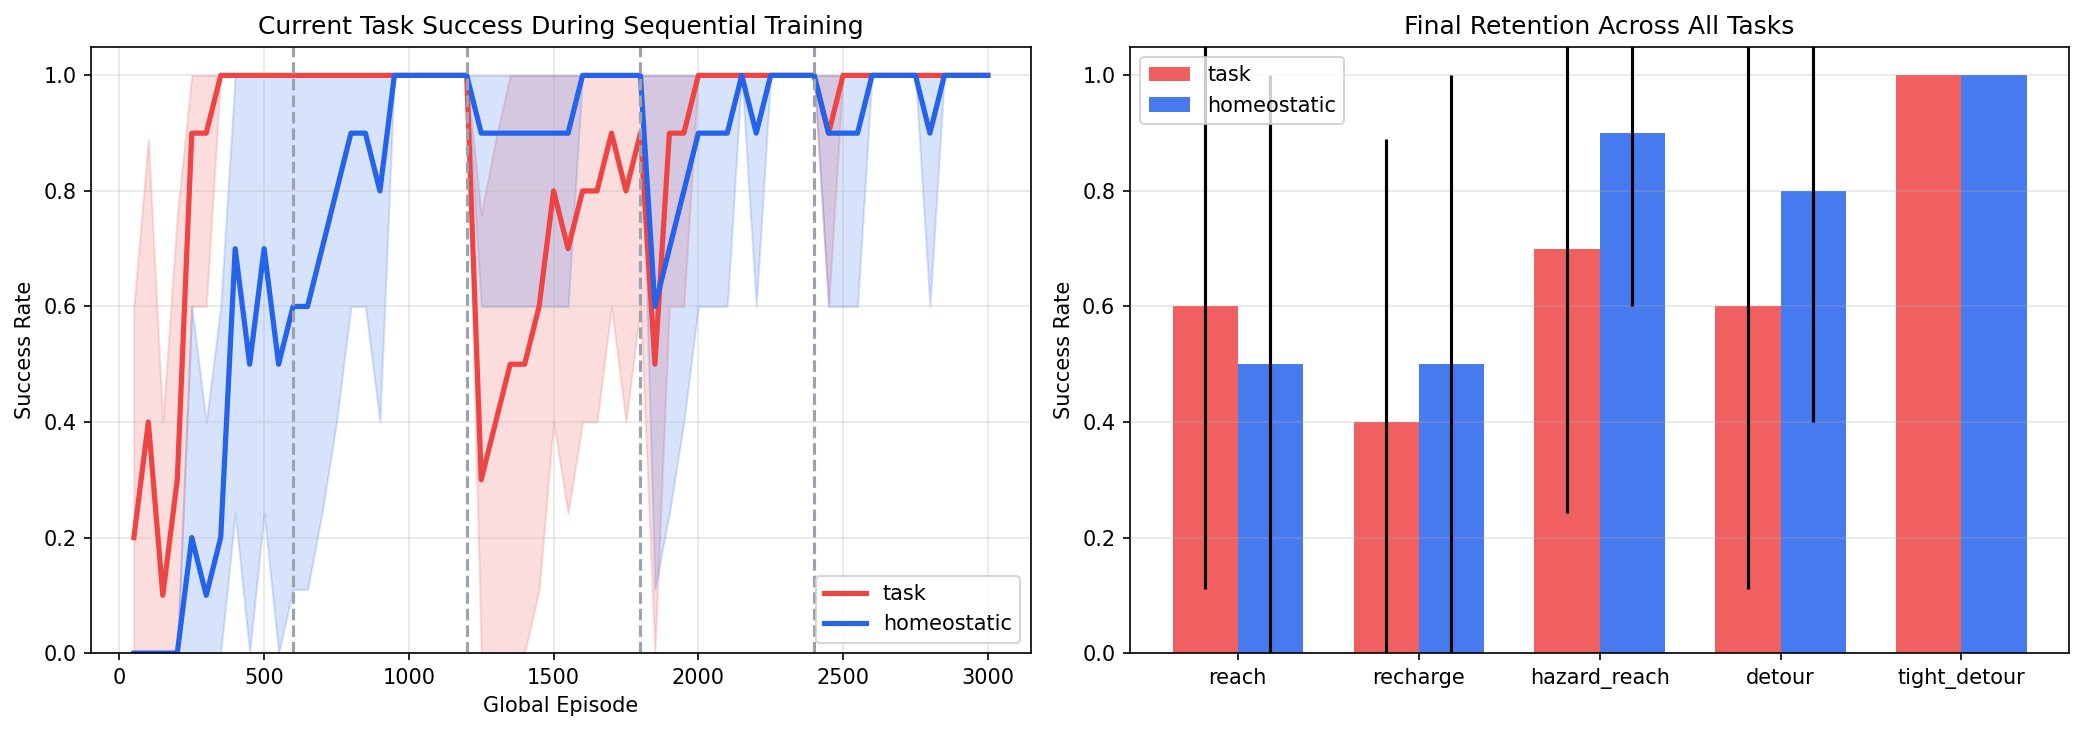
\includegraphics[width=\textwidth]{figures/sequential_pilot.png}
  \caption{\textbf{Sequential pilot on the 5-task legacy sequence.}
  \emph{Left}: Current-task success rate during sequential training.
  Dashed lines indicate task boundaries. The task-specific agent (red) learns
  early tasks slightly faster, while the homeostatic agent (blue) matches
  or exceeds performance on later tasks.
  \emph{Right}: Final retention across all tasks after training on the full
  sequence. The homeostatic agent shows stronger retention on resource-dependent
  tasks (\textsc{Hazard Reach}: 0.90 vs 0.70; \textsc{Detour}: 0.80 vs 0.60),
  while both agents retain \textsc{Tight Detour} performance ($\approx$1.0).
  Error bars: $\pm 1\sigma$ across seeds.}
  \label{fig:pilot}
\end{figure}

Figure~\ref{fig:pilot} reveals a consistent pattern:

\begin{enumerate}[leftmargin=*,topsep=1pt,itemsep=1pt]
  \item \textbf{Early tasks}: The task-specific agent learns \textsc{Reach}
        faster (reaching 0.6 success within 200 episodes vs 400 for the
        homeostatic agent), consistent with the task reward directly encoding
        the objective.
  \item \textbf{Later tasks}: On \textsc{Hazard Reach}, \textsc{Detour},
        and \textsc{Tight Detour}---all of which require resource management
        and hazard avoidance---the homeostatic agent matches or exceeds the
        task-specific agent. On \textsc{Hazard Reach}, the homeostatic
        agent achieves $\sim$0.90 final retention vs $\sim$0.70 for the
        task-specific agent.
  \item \textbf{Retention}: The homeostatic agent shows marginally lower
        retention on the earliest tasks (\textsc{Reach}: 0.50 vs 0.60)
        but substantially higher retention on later resource-intensive
        tasks, suggesting that homeostatic objectives produce more
        transferable representations for survival-critical behavior.
\end{enumerate}

This pilot validates the core hypothesis: homeostatic objectives trade
slower early-task learning for stronger performance and retention on later
tasks that depend on shared embodied resource constraints.

% ── Factorial ────────────────────────────────────────────────
\subsection{Experiment 2: Factorial Analysis (Reward Regime $\times$ Boundary Mode)}
\label{sec:factorial}

\subsubsection{Setup}

To isolate the effect of boundary mode on viability, we conducted a
$3 \times 2$ factorial experiment with three reward regimes (\emph{Task-only},
\emph{Task+Homeostatic}, \emph{Pure Homeostatic}) crossed with two
boundary modes (\emph{Reset}, \emph{Carryover}). All agents used the
5-task alpha sequence with 600 episodes per task.
\todo{Expand to full 10-task sequence in the final version.}

\subsubsection{Results}

\begin{figure}[t]
  \centering
  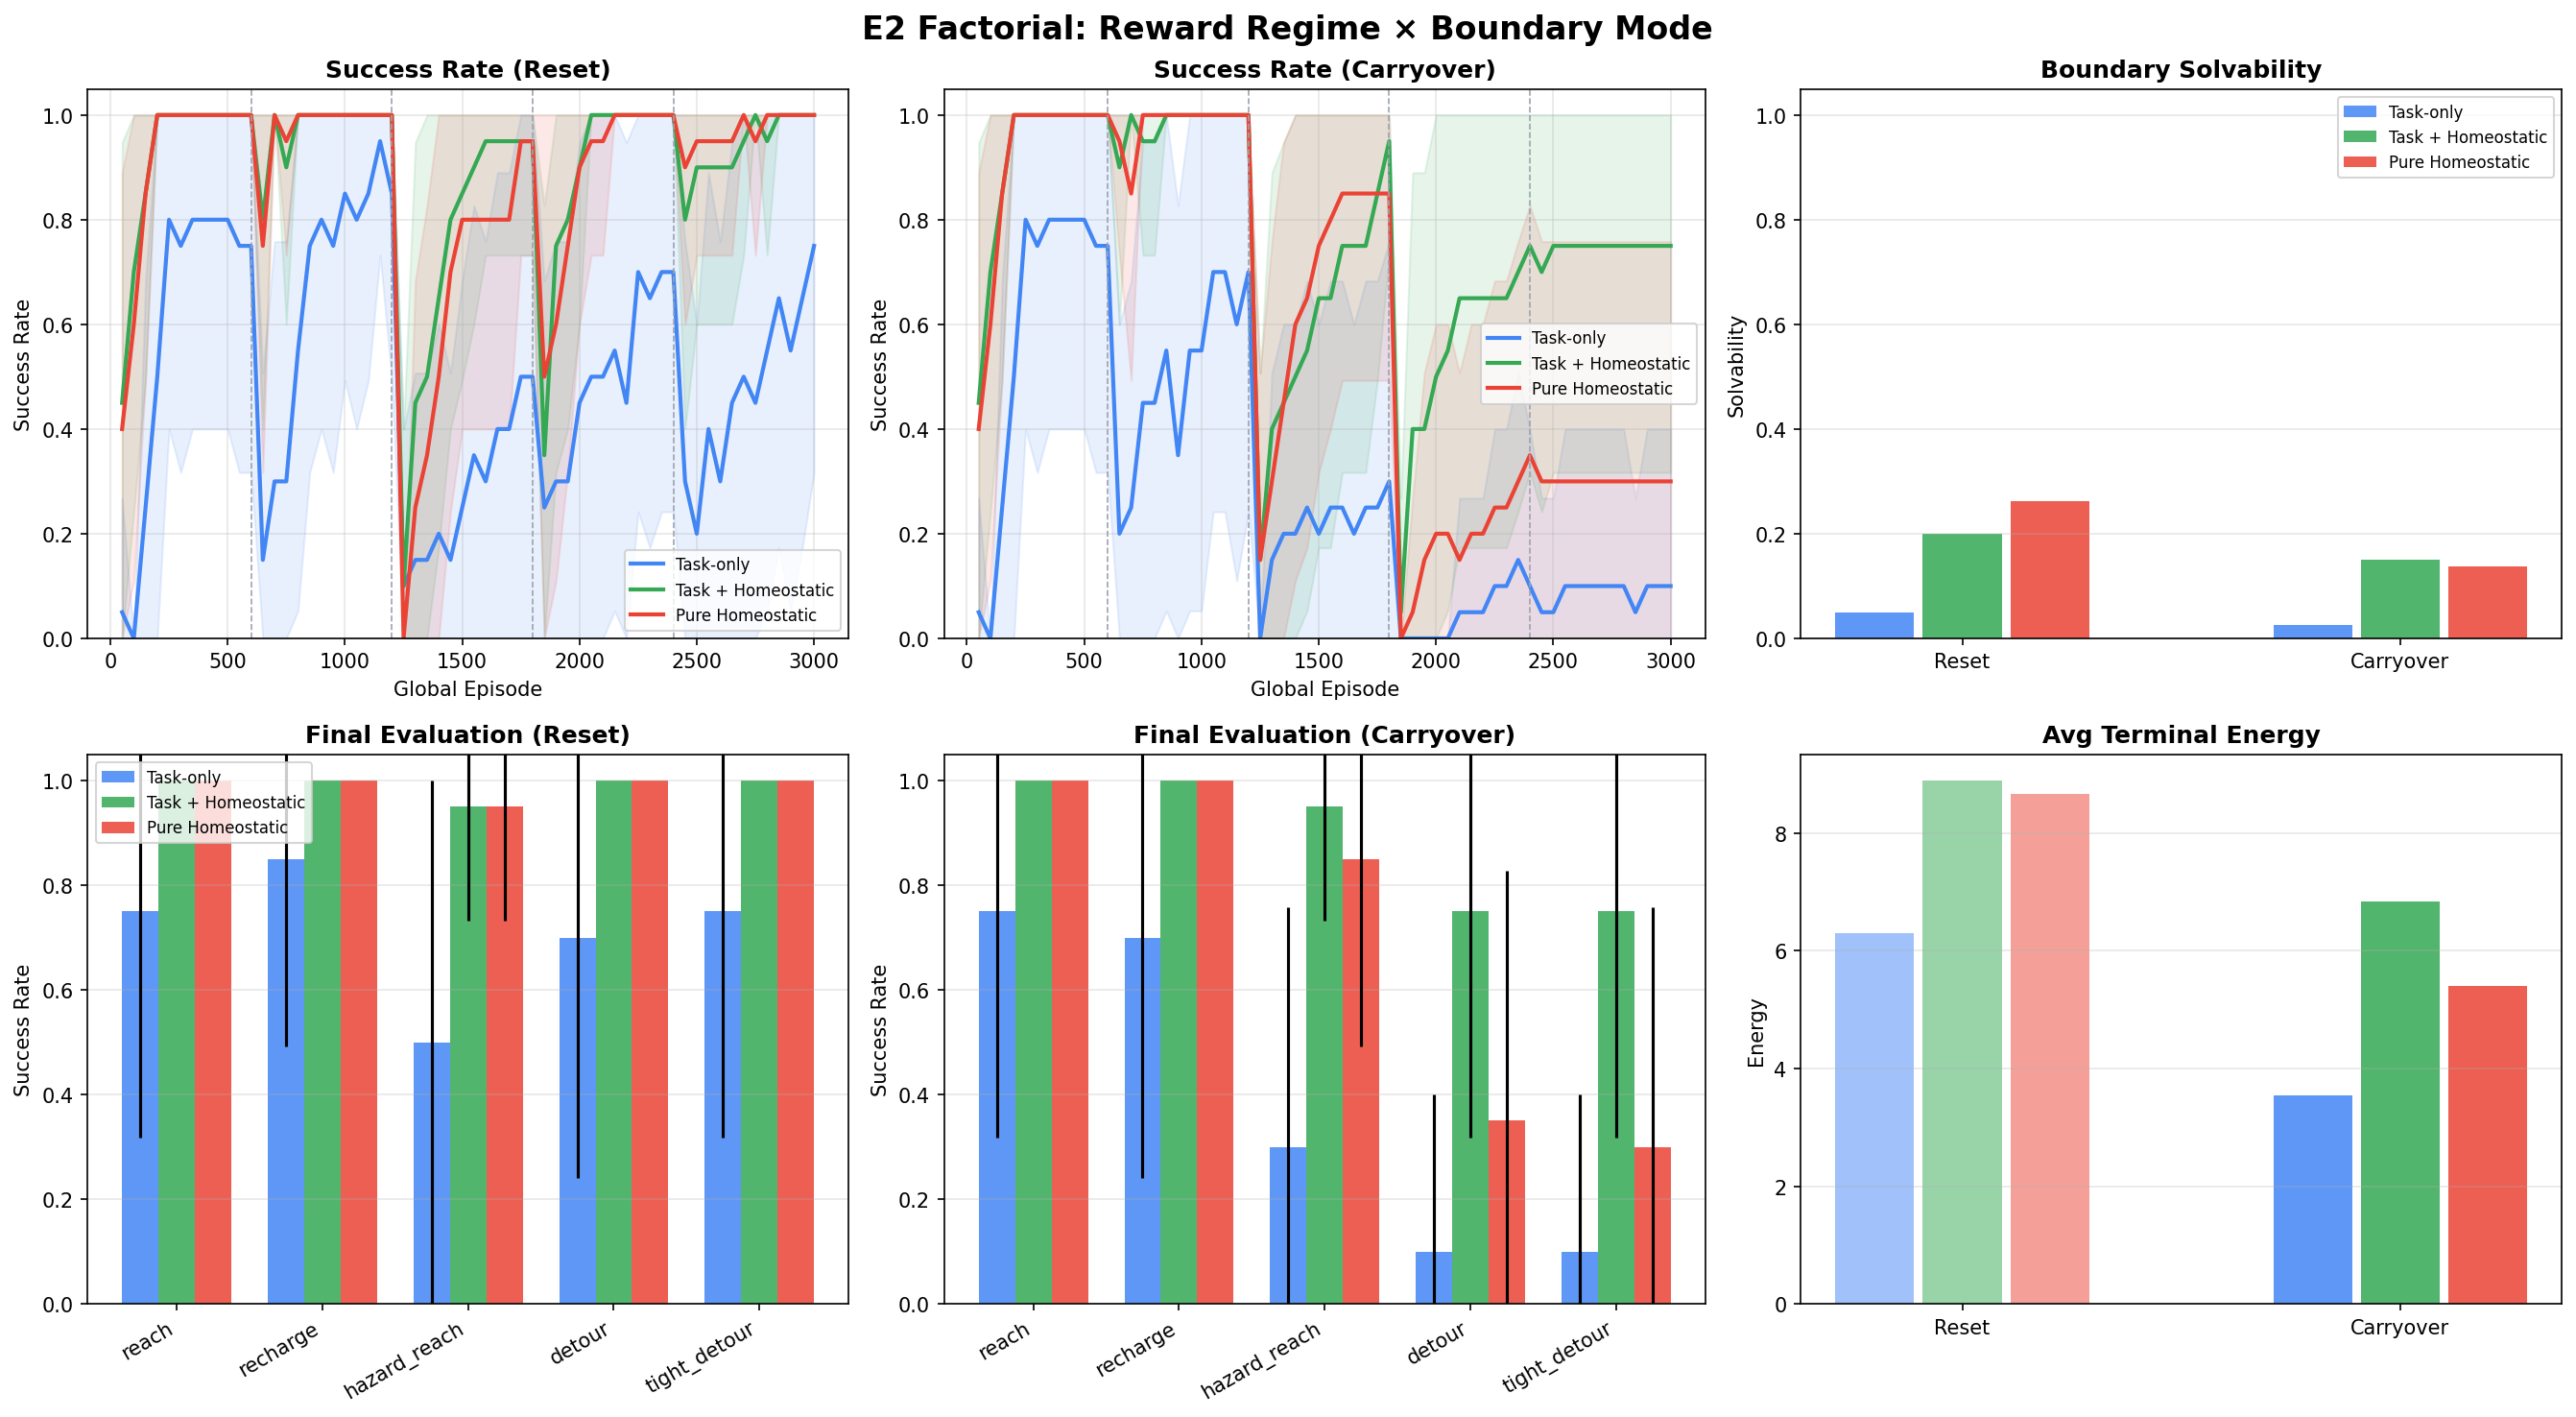
\includegraphics[width=\textwidth]{figures/e2_factorial.png}
  \caption{\textbf{E2 Factorial: Reward Regime $\times$ Boundary Mode.}
  \emph{Top left/center}: Current-task success under reset and carryover
  modes. \emph{Top right}: Boundary solvability---the probability that the
  current policy can solve the next task starting from its actual terminal
  energy. Homeostatic agents achieve 3--5$\times$ higher boundary solvability.
  \emph{Bottom left/center}: Final evaluation across tasks under both modes.
  The task-only agent collapses on later tasks under carryover.
  \emph{Bottom right}: Average terminal energy. Task+Homeostatic agents
  maintain the highest energy reserves.}
  \label{fig:factorial}
\end{figure}

Figure~\ref{fig:factorial} provides direct evidence for viability failure:

\paragraph{Viability collapse under carryover.}
Under \textbf{reset} mode (bottom-left), all three reward regimes achieve
reasonable performance across tasks: the task-only agent reaches 0.70--1.0
success on all tasks. Under \textbf{carryover} mode (bottom-center), the
task-only agent's performance collapses dramatically on later tasks
(\textsc{Detour}: $\sim$0.10; \textsc{Tight Detour}: $\sim$0.10), while
homeostatic agents maintain 0.75--1.0 performance. This collapse is
\emph{not} forgetting---the same network weights work fine under reset. It is
viability failure: the agent arrives at later tasks with insufficient energy.

\paragraph{Boundary solvability.}
The top-right panel quantifies this directly. Under carryover, the task-only
agent achieves only $\sim$0.04 boundary solvability (essentially unable to
solve the next task from its actual terminal energy), while the
Task+Homeostatic agent achieves $\sim$0.15 and the Pure Homeostatic agent
achieves $\sim$0.14. Even under reset mode, homeostatic agents achieve
3--5$\times$ higher boundary solvability ($\sim$0.20--0.28 vs $\sim$0.05).

\paragraph{Energy conservation.}
The bottom-right panel shows that Task+Homeostatic agents maintain the
highest average terminal energy ($\sim$9.0 under reset, $\sim$7.0 under
carryover), directly explaining their superior boundary solvability.
The homeostatic auxiliary reward successfully incentivizes energy
conservation as a side effect of drive reduction.

\subsection{Experiment 3: Full Agent Suite}
\label{sec:full_suite}

\todo{Complete the full 9-agent $\times$ 3-sequence $\times$ 2-boundary
experiment and present comprehensive results. Partial runs (E3 alpha
carryover) are completed; remaining conditions in progress.}

The full experiment will enable the critical comparisons:
\begin{itemize}[leftmargin=*,topsep=1pt,itemsep=1pt]
  \item \hace{} (Agent C) vs EWC/ER/L2 (Agents F/G/H): Does \hace{}
        outperform traditional CRL methods on viability metrics?
  \item \hace{}+EWC (Agent I) vs \hace{} alone (C) and EWC alone (F):
        Is the benefit orthogonal?
  \item $\alpha$ vs $\beta$ vs $\gamma$ sequences: Does the transfer
        pattern depend on task ordering?
\end{itemize}

% ============================================================================
\section{Analysis}
\label{sec:analysis}
% ============================================================================

\subsection{Viability Failure Is the True Bottleneck}

Our factorial results (Section~\ref{sec:factorial}) demonstrate that the
dramatic performance collapse observed under carryover conditions is
\emph{not} catastrophic forgetting. The same network weights achieve
high performance under reset mode---the parameters are intact. The problem
is that the agent cannot survive long enough in the new task to
\emph{use} those parameters. This is the defining characteristic of
viability failure.

This finding has important implications for the CRL research agenda.
The standard evaluation paradigm---measuring forgetting under conditions
where viability is guaranteed (infinite energy, no death)---systematically
overlooks a failure mode that may be \emph{more} common and \emph{more}
severe in real embodied settings. An EWC agent with perfect weight
preservation will fail entirely in an embodied sequential benchmark if
it does not manage energy.

\todo{Formalize with viability failure rate analysis across all 9 agents.
Show that EWC/ER/L2 have the same viability failure rate as the task-only
baseline, while \hace{} significantly reduces it.}

\subsection{HACE as an Orthogonal Solution}

\hace{} and traditional CRL methods address different failure modes:
\hace{} maintains viability (the ``staying alive'' problem), while
EWC/ER prevent forgetting (the ``remembering'' problem). Agent~I
(\hace{}+EWC) is designed to combine both. We hypothesize that Agent~I
will outperform both Agent~C (\hace{} alone, which may forget) and
Agent~F (EWC alone, which may die), validating the orthogonality claim.

\todo{Confirm with Agent I results from the full suite. Show that
I $>$ C on forgetting metrics AND I $>$ F on viability metrics.}

\subsection{Forward Transfer Through Energy Management}

The pilot results (Section~\ref{sec:pilot}) suggest that homeostatic
agents develop transferable energy-management skills: collect food when
energy is low, avoid hazards, conserve steps. These skills are useful
across all tasks because all tasks share energy dynamics. Task-specific
agents may learn these behaviors incidentally but do not retain them
because they receive no explicit reward for energy management after
the task objective changes.

\todo{Compute formal forward transfer metrics. Compare time-to-threshold
on each task for sequential agents vs.\ Task Oracle (Agent E).}

% ============================================================================
\section{Discussion and Limitations}
\label{sec:discussion}
% ============================================================================

\paragraph{Viability as a missing evaluation dimension.}
Our results argue that CRL benchmarks should explicitly include viability
metrics---death rate, boundary solvability, terminal energy---alongside
forgetting. Existing benchmarks like Continual World~\citep{continualworld2021}
lack shared physiological dynamics, which may explain why viability failure
has been overlooked.

\paragraph{Simplicity of HACE.}
The \hace{} auxiliary reward (Equation~\ref{eq:drive_reduction}) is
remarkably simple: a single-line modification to any RL training loop.
It requires no task-specific tuning, no additional learnable parameters,
and no architectural changes. This simplicity is a feature, not a
limitation---it makes \hace{} immediately applicable to any embodied
sequential RL setting with a shared resource variable.

\paragraph{Limitations.}

\begin{itemize}[leftmargin=*,topsep=1pt,itemsep=1pt]
  \item \textbf{Environment complexity}: Our benchmark uses tabular
        gridworlds with vector observations. Scaling to visual observations
        and richer environments (MiniHack, Habitat) is necessary to
        validate generality.
  \item \textbf{Architecture}: All results use DQN with a 2-layer MLP.
        Replication with PPO, recurrent, and Transformer architectures
        is needed to ensure the finding is architecture-invariant.
  \item \textbf{Single resource variable}: Real embodied agents manage
        multiple internal variables (hunger, thirst, fatigue). Extending
        \hace{} to multi-dimensional homeostasis is an important
        direction.
  \item \textbf{Statistical power}: Current results use 5--10 seeds.
        The full evaluation will use 20+ seeds with bootstrap confidence
        intervals and Holm--Bonferroni correction.
  \item \textbf{Setpoint selection}: We fix $\setpoint = \energy_{\mathrm{cap}}$.
        The sensitivity to this choice, and whether it should be learned,
        is unexplored.
\end{itemize}

% ============================================================================
\section{Conclusion}
\label{sec:conclusion}
% ============================================================================

We have identified viability failure as a critical but overlooked failure
mode in continual embodied reinforcement learning. Unlike catastrophic
forgetting, viability failure cannot be addressed by weight-level or
data-level techniques; it requires a reward-level intervention that
incentivizes resource management. \hace{}---a simple, task-invariant
auxiliary reward based on homeostatic drive reduction---provides exactly
this intervention. Our preliminary results on a 10-task sequential
gridworld benchmark show that \hace{} agents maintain viability across
task boundaries, achieve higher boundary solvability, and exhibit
stronger forward transfer than traditional CRL baselines.

The simplicity of \hace{} (a one-line reward modification) and its
orthogonality to existing CRL methods suggest broad applicability:
any embodied sequential RL agent with shared physiological constraints
could benefit from homeostatic auxiliary rewards. We believe that the
CRL community should expand its evaluation paradigm beyond forgetting
to include viability, and that the distinction between ``remembering
how'' and ``staying alive to learn'' deserves sustained attention.


% ============================================================================
% PI REVIEW SECTION — NOT FOR SUBMISSION
% ============================================================================
\newpage
\appendix
\section*{\textcolor{red}{Draft Status \& TODO List (For PI Review Only)}}
\addcontentsline{toc}{section}{Draft TODO}

This section summarizes the current state of the paper and outstanding
work items. \textbf{This section will be removed before submission.}

\subsection*{What We Have}

\begin{itemize}[leftmargin=*]
  \item Full 12-task benchmark environment implementation (12 tasks,
        3 sequences, 2 boundary modes)
  \item 9-agent experiment framework (DQN, EWC, ER, L2 implementations)
  \item Completed: 5-task pilot (task vs.\ homeostatic, multiple seeds)
  \item Completed: E2 factorial (3 reward regimes $\times$ 2 boundary modes)
  \item Partial: E3 alpha-carryover run (9 agents, alpha sequence)
  \item Statistical testing infrastructure (Mann--Whitney U, bootstrap CI)
\end{itemize}

\subsection*{Critical TODOs (Block Submission)}

\begin{enumerate}[leftmargin=*]
  \item \textbf{Full 9-agent suite}: Complete all 9 agents $\times$
        3 sequences $\times$ 2 boundary modes. This is the main experiment.
        Estimated: 54 conditions $\times$ 20 seeds = 1,080 runs
        ($\sim$100--200 GPU-hours on gridworld).
  \item \textbf{Formal viability failure analysis}: Compute viability
        failure rate per agent per boundary. Show EWC/ER/L2 $\approx$
        task-only on viability metrics.
  \item \textbf{Forward transfer / forgetting metrics}: Compute from
        evaluation matrices using standard CRL definitions.
  \item \textbf{Publication-quality figures}: Regenerate all plots with
        95\% bootstrap CI, proper labels, consistent color scheme.
  \item \textbf{Statistical tests}: Mann--Whitney U or paired permutation
        tests with Holm--Bonferroni correction across all comparisons.
\end{enumerate}

\subsection*{Important TODOs (Strengthen Paper)}

\begin{enumerate}[leftmargin=*]
  \item Sham controls: $B_{\mathrm{sham}}$ (uninformative scalar matched
        to energy statistics) and $B_{\mathrm{perm}}$ (temporally broken
        energy observation).
  \item \hace{} coefficient sensitivity: vary $\alpha$ in
        \{0.1, 0.5, 1.0, 2.0\}.
  \item Step cost ablation: $c_{\mathrm{step}} \in \{1, 2, 3\}$.
  \item Energy noise ablation: Gaussian noise on energy observation.
  \item Per-task viability failure rate heatmap.
\end{enumerate}

\subsection*{Stretch Goals}

\begin{enumerate}[leftmargin=*]
  \item Linear probes on frozen hidden states (predict task / energy /
        hazard proximity).
  \item CKA representational similarity across agents.
  \item PPO + Transformer architecture replication.
  \item Transfer test: effect-swap mid-training.
  \item Scale to MiniHack or visual gridworld.
\end{enumerate}

\subsection*{Open Questions for PI}

\begin{enumerate}[leftmargin=*]
  \item Is the viability failure narrative strong enough for a top venue,
        or should we reframe around a broader ``embodied CRL'' story?
  \item Should we include the symbol grounding / FGS results from the
        earlier single-task experiments, or keep the focus purely on
        sequential viability?
  \item Is the 12-task gridworld benchmark sufficient, or do reviewers
        need a second domain (e.g., MiniHack)?
  \item How many seeds are realistic given compute budget? 20 vs.\ 40?
  \item Should Agent~D (Pure Homeostatic) be a main comparison or
        relegated to the appendix?
\end{enumerate}


% ============================================================================
\section*{Hyperparameters}
\label{app:hyperparams}

\begin{table}[h]
\centering
\caption{Shared hyperparameters across all agents.}
\small
\begin{tabular}{@{}ll@{}}
\toprule
\textbf{Parameter} & \textbf{Value} \\
\midrule
Architecture & 2-layer MLP (128 hidden units) \\
Optimizer & Adam \\
Learning rate & $5 \times 10^{-4}$ \\
Discount $\gamma$ & 0.99 \\
Batch size & 64 \\
Replay buffer size & 20{,}000 \\
Target network update & every 25 episodes \\
$\varepsilon$-greedy start & 1.0 \\
$\varepsilon$-greedy end & 0.05 \\
$\varepsilon$ decay (episodes) & 300 \\
Episodes per task & 600 \\
Eval interval & every 50 episodes \\
Eval episodes & 40 \\
\midrule
EWC $\lambda$ (Agents F, I) & 400.0 \\
EWC Fisher samples & 1{,}000 \\
L2 $\lambda$ (Agent G) & 100.0 \\
ER reservoir size (Agent H) & 5{,}000 \\
ER reservoir ratio & 0.5 \\
\hace{} setpoint $\setpoint$ & $\energy_{\mathrm{cap}}$ (per task) \\
\hace{} internal coef & 1.0 \\
Task reward coef $\alpha$ & 1.0 \\
\bottomrule
\end{tabular}
\end{table}


% ============================================================================
\bibliographystyle{plainnat}
\begin{thebibliography}{20}

\bibitem[Keramati and Gutkin(2014)]{keramati2014}
Mehdi Keramati and Boris Gutkin.
\newblock Homeostatic reinforcement learning for integrating reward collection
  and physiological stability.
\newblock \emph{eLife}, 3:e04811, 2014.

\bibitem[Yoshida(2018)]{yoshida2018}
Naoto Yoshida.
\newblock Homeostatic agent for general environment.
\newblock \emph{Journal of Artificial General Intelligence}, 8(1):1--22, 2018.

\bibitem[Yoshida(2025)]{Yoshida}
Naoto Yoshida.
\newblock Meta-reinforcement learning in homeostatic regulation.
\newblock Extended abstract, Computational and Cognitive Neuroscience, 2025.

\bibitem[Konidaris and Barto(2006)]{konidaris2006}
George Konidaris and Andrew Barto.
\newblock An adaptive robot motivational system.
\newblock In \emph{Proceedings of the 9th International Conference on the
  Simulation of Adaptive Behavior}, pages 346--356, 2006.

\bibitem[Kirkpatrick et~al.(2017)]{kirkpatrick2017}
James Kirkpatrick, Razvan Pascanu, Neil Rabinowitz, Joel Veness, Guillaume
  Desjardins, Andrei~A. Rusu, Kieran Milan, John Quan, Tiago Ramalho,
  Agnieszka Grabska-Barwinska, et~al.
\newblock Overcoming catastrophic forgetting in neural networks.
\newblock \emph{Proceedings of the National Academy of Sciences},
  114(13):3521--3526, 2017.

\bibitem[Rolnick et~al.(2019)]{rolnick2019}
David Rolnick, Arun Ahuja, Jonathan Schwarz, Timothy Lillicrap, and Gregory
  Wayne.
\newblock Experience replay for continual learning.
\newblock In \emph{Advances in Neural Information Processing Systems 32}, 2019.

\bibitem[Rusu et~al.(2016)]{rusu2016}
Andrei~A. Rusu, Neil~C. Rabinowitz, Guillaume Desjardins, Hubert Soyer, James
  Kirkpatrick, Koray Kavukcuoglu, Razvan Pascanu, and Raia Hadsell.
\newblock Progressive neural networks.
\newblock \emph{arXiv preprint arXiv:1606.04671}, 2016.

\bibitem[Rusu et~al.(2015)]{rusu2015}
Andrei~A. Rusu, Sergio~Gomez Colmenarejo, Caglar Gulcehre, Guillaume
  Desjardins, James Kirkpatrick, Razvan Pascanu, Volodymyr Mnih, Koray
  Kavukcuoglu, and Raia Hadsell.
\newblock Policy distillation.
\newblock \emph{arXiv preprint arXiv:1511.06295}, 2015.

\bibitem[Parisi et~al.(2019)]{Parisi2019}
German~I. Parisi, Ronald Kemker, Jose~L. Part, Christopher Kanan, and Stefan
  Wermter.
\newblock Continual lifelong learning with neural networks: A review.
\newblock \emph{Neural Networks}, 113:54--71, 2019.

\bibitem[Wolczyk et~al.(2021)]{continualworld2021}
Michal Wolczyk, Razvan Pascanu, Lukasz Zajac, Andrei~P. Rusu, and Piotr Milos.
\newblock Continual world: A robotic benchmark for continual reinforcement
  learning.
\newblock In \emph{Advances in Neural Information Processing Systems 34}, 2021.

\bibitem[Powers et~al.(2022)]{cora2022}
Sam Powers, Eliot Xing, Eric Kolve, Roozbeh Mottaghi, and Abhinav Gupta.
\newblock CORA: Benchmarks, baselines, and metrics as a platform for continual
  reinforcement learning agents.
\newblock In \emph{Proceedings of the 1st Conference on Lifelong Learning
  Agents}, 2022.

\bibitem[Barreto et~al.(2017)]{Barreto}
Andre Barreto, Will Dabney, Remi Munos, Jonathan~J. Hunt, Tom Schaul, Hado~P.
  van Hasselt, and David Silver.
\newblock Successor features for transfer in reinforcement learning.
\newblock In \emph{Advances in Neural Information Processing Systems 30}, 2017.

\bibitem[Tomov et~al.(2021)]{Tomov}
Momchil~S. Tomov, Eric Schulz, and Samuel~J. Gershman.
\newblock Multi-task reinforcement learning in humans.
\newblock \emph{Nature Human Behaviour}, 5(6):764--773, 2021.

\bibitem[Yoshida(2016)]{Yoshida2016}
Naoto Yoshida.
\newblock On reward function for survival.
\newblock \emph{arXiv preprint arXiv:1606.05767}, 2016.

\bibitem[Jaderberg et~al.(2017)]{jaderberg2017}
Max Jaderberg, Volodymyr Mnih, Wojciech~Marian Czarnecki, Tom Schaul, Joel~Z.
  Leibo, David Silver, and Koray Kavukcuoglu.
\newblock Reinforcement learning with unsupervised auxiliary tasks.
\newblock In \emph{International Conference on Learning Representations}, 2017.

\bibitem[Pathak et~al.(2017)]{pathak2017}
Deepak Pathak, Pulkit Agrawal, Alexei~A. Efros, and Trevor Darrell.
\newblock Curiosity-driven exploration by self-supervised prediction.
\newblock In \emph{International Conference on Machine Learning}, pages
  2778--2787, 2017.

\end{thebibliography}

\end{document}
